\documentclass[11pt,preprint]{elsarticle}

\usepackage{lmodern}
%%%% My spacing
\usepackage{setspace}
\setstretch{1.2}
\DeclareMathSizes{12}{14}{10}{10}

% Wrap around which gives all figures included the [H] command, or places it "here". This can be tedious to code in Rmarkdown.
\usepackage{float}
% The [H] wrapper for figures is switched off, so that figures float to the top or bottom of a page as set by fig.pos in the Rmd and pages are not left half empty
% \let\origfigure\figure
% \let\endorigfigure\endfigure
% \renewenvironment{figure}[1][2] {
%     \expandafter\origfigure\expandafter[H]
% } {
%     \endorigfigure
% }

\let\origtable\table
\let\endorigtable\endtable
\renewenvironment{table}[1][2] {
    \expandafter\origtable\expandafter[H]
} {
    \endorigtable
}


\usepackage{ifxetex,ifluatex}
\usepackage{fixltx2e} % provides \textsubscript
\ifnum 0\ifxetex 1\fi\ifluatex 1\fi=0 % if pdftex
  \usepackage[T1]{fontenc}
  \usepackage[utf8]{inputenc}
\else % if luatex or xelatex
  \ifxetex
    \usepackage{mathspec}
    \usepackage{xltxtra,xunicode}
  \else
    \usepackage{fontspec}
  \fi
  \defaultfontfeatures{Mapping=tex-text,Scale=MatchLowercase}
  \newcommand{\euro}{€}
\fi

\usepackage{amssymb, amsmath, amsthm, amsfonts}

\def\bibsection{\section*{References}} %%% Make "References" appear before bibliography


\usepackage[numbers]{natbib}

\usepackage{longtable}
\usepackage[margin=2.3cm,bottom=2cm,top=2.5cm, includefoot]{geometry}
\usepackage{fancyhdr}
\usepackage[bottom, hang, flushmargin]{footmisc}
\usepackage{graphicx}
\numberwithin{equation}{section}
\numberwithin{figure}{section}
\numberwithin{table}{section}
\setlength{\parindent}{0cm}
\setlength{\parskip}{1.3ex plus 0.5ex minus 0.3ex}
\usepackage{textcomp}
\renewcommand{\headrulewidth}{0.2pt}
\renewcommand{\footrulewidth}{0.3pt}

\usepackage{array}
\newcolumntype{x}[1]{>{\centering\arraybackslash\hspace{0pt}}p{#1}}

%%%%  Remove the "preprint submitted to" part. Don't worry about this either, it just looks better without it:
\makeatletter
\def\ps@pprintTitle{%
  \let\@oddhead\@empty
  \let\@evenhead\@empty
  \let\@oddfoot\@empty
  \let\@evenfoot\@oddfoot
}
\makeatother

 \def\tightlist{} % This allows for subbullets!

\usepackage{hyperref}
\hypersetup{breaklinks=true,
            bookmarks=true,
            colorlinks=true,
            citecolor=blue,
            urlcolor=blue,
            linkcolor=blue,
            pdfborder={0 0 0}}


% The following packages allow huxtable to work:
\usepackage{siunitx}
\usepackage{multirow}
\usepackage{hhline}
\usepackage{calc}
\usepackage{tabularx}
\usepackage{booktabs}
\usepackage{caption}


\newenvironment{columns}[1][]{}{}

\newenvironment{column}[1]{\begin{minipage}{#1}\ignorespaces}{%
\end{minipage}
\ifhmode\unskip\fi
\aftergroup\useignorespacesandallpars}

\def\useignorespacesandallpars#1\ignorespaces\fi{%
#1\fi\ignorespacesandallpars}

\makeatletter
\def\ignorespacesandallpars{%
  \@ifnextchar\par
    {\expandafter\ignorespacesandallpars\@gobble}%
    {}%
}
\makeatother


% definitions for citeproc citations
\NewDocumentCommand\citeproctext{}{}
\NewDocumentCommand\citeproc{mm}{%
\href{\#cite.\detokenize{#1}}{#2}\nocite{#1}}

\makeatletter
% allow citations to break across lines
\let\@cite@ofmt\@firstofone
% avoid brackets around text for \cite:
\def\@biblabel#1{}
\def\@cite#1#2{{#1\if@tempswa , #2\fi}}
\makeatother
\newlength{\cslhangindent}
\setlength{\cslhangindent}{1.5em}
\newlength{\csllabelwidth}
\setlength{\csllabelwidth}{3em}
\newenvironment{CSLReferences}[2] % #1 hanging-indent, #2 entry-spacing
{\begin{list}{}{%
	\setlength{\itemindent}{0pt}
	\setlength{\leftmargin}{0pt}
	\setlength{\parsep}{0pt}
	% turn on hanging indent if param 1 is 1
	\ifodd #1
	\setlength{\leftmargin}{\cslhangindent}
	\setlength{\itemindent}{-1\cslhangindent}
	\fi
	% set entry spacing
	\setlength{\itemsep}{#2\baselineskip}}}
{\end{list}}

\usepackage{calc}
\newcommand{\CSLBlock}[1]{\hfill\break\parbox[t]{\linewidth}{\strut\ignorespaces#1\strut}}
\newcommand{\CSLLeftMargin}[1]{\parbox[t]{\csllabelwidth}{\strut#1\strut}}
\newcommand{\CSLRightInline}[1]{\parbox[t]{\linewidth - \csllabelwidth}{\strut#1\strut}}
\newcommand{\CSLIndent}[1]{\hspace{\cslhangindent}#1}


\urlstyle{same}  % don't use monospace font for urls
\setlength{\parindent}{0pt}
\setlength{\parskip}{6pt plus 2pt minus 1pt}
\setlength{\emergencystretch}{3em}  % prevent overfull lines
\setcounter{secnumdepth}{5}

%%% Use protect on footnotes to avoid problems with footnotes in titles
\let\rmarkdownfootnote\footnote%
\def\footnote{\protect\rmarkdownfootnote}
\IfFileExists{upquote.sty}{\usepackage{upquote}}{}

%%% Include extra packages specified by user
\renewcommand{\topfraction}{0.9}
\renewcommand{\bottomfraction}{0.8}
\renewcommand{\textfraction}{0.07}
\renewcommand{\floatpagefraction}{0.8}
\setcounter{topnumber}{2}
\setcounter{bottomnumber}{2}
\setcounter{totalnumber}{3}
\usepackage{placeins}

%%% Hard setting column skips for reports - this ensures greater consistency and control over the length settings in the document.
%% page layout
%% paragraphs
\setlength{\baselineskip}{12pt plus 0pt minus 0pt}
\setlength{\parskip}{12pt plus 0pt minus 0pt}
\setlength{\parindent}{0pt plus 0pt minus 0pt}
%% floats
\setlength{\floatsep}{12pt plus 0 pt minus 0pt}
\setlength{\textfloatsep}{20pt plus 0pt minus 0pt}
\setlength{\intextsep}{14pt plus 0pt minus 0pt}
\setlength{\dbltextfloatsep}{20pt plus 0pt minus 0pt}
\setlength{\dblfloatsep}{14pt plus 0pt minus 0pt}
%% maths
\setlength{\abovedisplayskip}{12pt plus 0pt minus 0pt}
\setlength{\belowdisplayskip}{12pt plus 0pt minus 0pt}
%% lists
\setlength{\topsep}{10pt plus 0pt minus 0pt}
\setlength{\partopsep}{3pt plus 0pt minus 0pt}
\setlength{\itemsep}{5pt plus 0pt minus 0pt}
\setlength{\labelsep}{8mm plus 0mm minus 0mm}
\setlength{\parsep}{\the\parskip}
\setlength{\listparindent}{\the\parindent}
%% verbatim
\setlength{\fboxsep}{5pt plus 0pt minus 0pt}



\begin{document}



\begin{frontmatter}  %

\title{Size and Risk in the Local Equity Market, a Comparison of Large,
Mid and Small Cap Indexes}

% Set to FALSE if wanting to remove title (for submission)




\author[Add1]{Diaz Sangeve}
\ead{24991422@sun.ac.za}





\address[Add1]{Stellenbosch University, Stellenbosch, South Africa}

\cortext[cor]{Corresponding author: Diaz Sangeve}

\begin{abstract}
\small{
This report compares the traits of the local large, mid and small cap
indexes against the Capped SWIX. The large-cap index is a concentrated,
resource-heavy portfolio that has become close to a copy of the
benchmark, with an active share of 13 percent in August 2026, and it
delivered the best risk-adjusted return and the shallowest drawdown
between 2015 and 2026. The small-cap index is the only one that differs
materially from the benchmark. Its domestic, property-heavy constituents
are the most volatile individually, yet they combine into the calmest
index, because their shocks are largely unrelated. That diversification
breaks down in crises and when the rand is volatile, and part of the
small caps' measured calm reflects stale prices in thinly traded stocks.
The mid-cap index has drifted towards the large caps in its holdings and
concentration, and has offered the weakest return with the least
favourable asymmetry between up and down markets.
}
\end{abstract}

\vspace{1cm}


\begin{keyword}
\footnotesize{
Size indexes \sep Concentration \sep Active share \sep Realised
volatility \sep Stratification \\
\vspace{0.3cm}
}
\footnotesize{
\textit{JEL classification} G11 \sep G12 \sep G15
}
\end{keyword}



\vspace{0.5cm}

\end{frontmatter}

\setcounter{footnote}{0}



%________________________
% Header and Footers
%%%%%%%%%%%%%%%%%%%%%%%%%%%%%%%%%
\pagestyle{fancy}
\chead{}
\rhead{}
\lfoot{}
\rfoot{\footnotesize Page \thepage}
\lhead{}
%\rfoot{\footnotesize Page \thepage } % "e.g. Page 2"
\cfoot{}

%\setlength\headheight{30pt}
%%%%%%%%%%%%%%%%%%%%%%%%%%%%%%%%%
%________________________

\headsep 35pt % So that header does not go over title




\section{\texorpdfstring{Introduction
\label{Intro}}{Introduction }}\label{introduction}

Size indexes are often treated as interchangeable slices of the same
market, differing only in the size of the companies they hold. This
report shows that the local large, mid and small cap indexes are
distinct portfolios, with different sector bets, levels of
concentration, distances from the benchmark, volatility structures and
responses to market stress. Section \ref{Data} describes the data,
Section \ref{Holdings} compares what each index holds, Section \ref{Vol}
measures the realised volatility of the constituents, Section
\ref{Returns} compares the risk and return profiles of the indexes and
Section \ref{Strat} stratifies their behaviour by market regime. Section
\ref{Conclusion} concludes.

\section{\texorpdfstring{Data and Approach
\label{Data}}{Data and Approach }}\label{data-and-approach}

\subsection{The Data and the Order of the
Analysis}\label{the-data-and-the-order-of-the-analysis}

This question compares the traits of the three local size indexes, the
large, mid and small caps, against the Capped SWIX as the full
benchmark. The analysis draws on two sources. The monthly constituent
file gives the holdings and weights of each index from January 2007,
which show what each index owns, how concentrated it is and how far it
departs from the benchmark. The daily stock returns, which start in
January 2015, are then applied to those holdings to measure how volatile
the constituents are and how much of that volatility survives once they
are combined into an index. The published daily returns of the Top 40,
Mid Cap and Small Cap indexes are used to measure each index's risk and
return profile through rolling returns, a comparison across sub-periods
and stratification by market conditions.

The section is ordered in three steps. It first establishes what each
index holds, through sector exposure, stock concentration and active
share. It then measures the realised volatility of the constituents and
the share of it that diversification removes. Finally, it asks how each
index has rewarded that risk over time and across calm and stressed
markets. Stocks without a sector in the constituent file are labelled
unclassified, and weights are rescaled to sum to one in every month,
since the reported weights do not always do so.

\section{\texorpdfstring{What the Indexes Hold
\label{Holdings}}{What the Indexes Hold }}\label{what-the-indexes-hold}

\subsection{Sector Exposure}\label{sector-exposure}

The first trait is what each index is exposed to. The figure stacks the
sector weights of every index through time, using the same sector
colours as Question 1, so that each panel shows the sector mix of one
index.

\begin{figure}[H]

{\centering 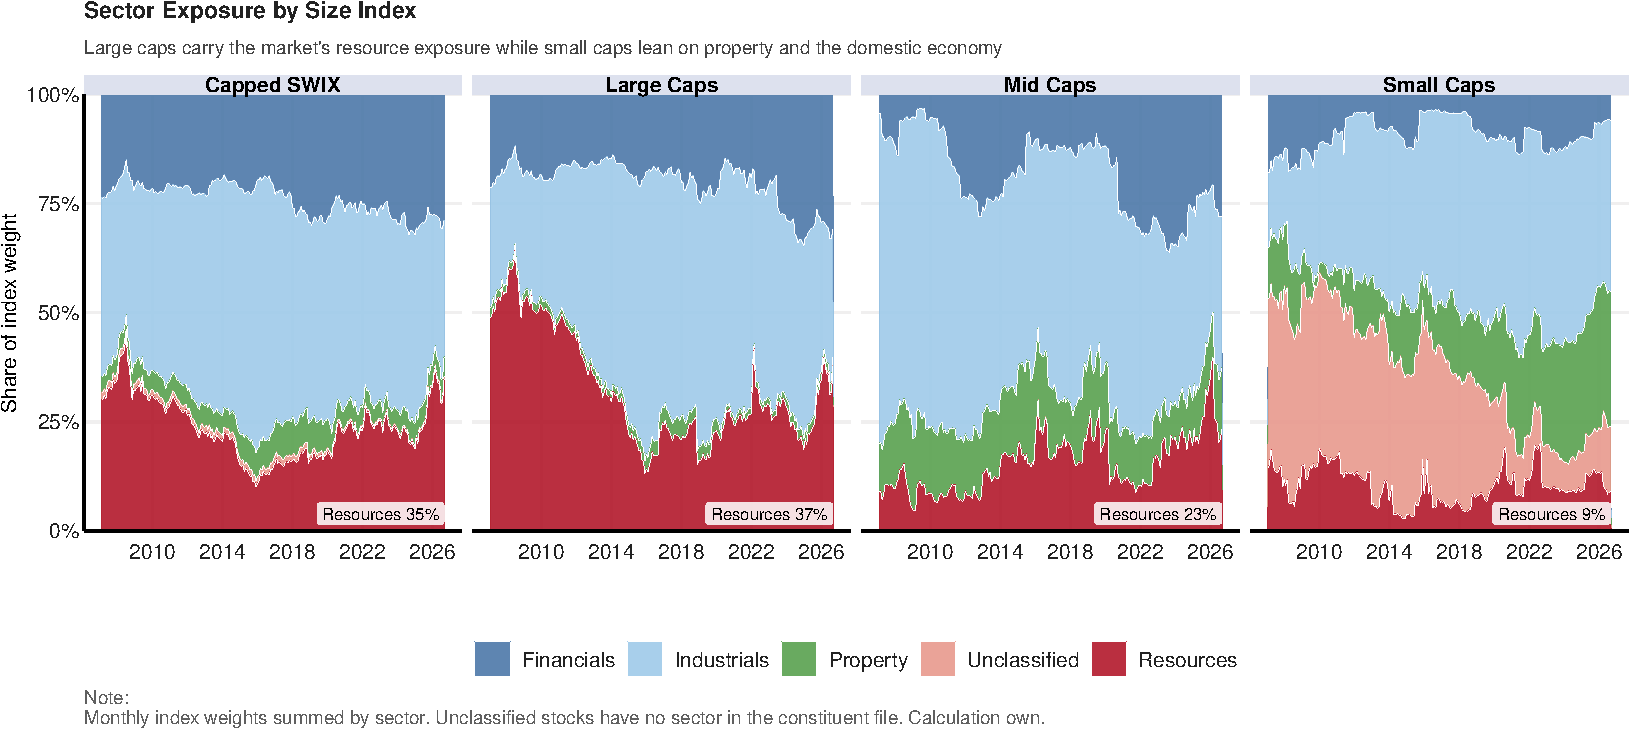
\includegraphics[width=1\linewidth]{Question2_files/figure-latex/q2_sectors-1} 

}

\caption{Sector Exposure by Size Index}\label{fig:q2_sectors}
\end{figure}

The three indexes are different bets on the South African economy. The
large-cap index carries most of the market's resource exposure, with
resources at 49 percent of the index in January 2007 and 37 percent in
August 2026, after the gold rally of 2026 lifted Gold Fields and
AngloGold Ashanti to the top of the index. Its returns therefore depend
heavily on global commodity prices and on the offshore earnings of its
largest industrials. The mid-cap index began the sample as an
industrials index, with 76 percent of its weight in that sector, and has
since spread across financials, resources and property. The small-cap
index is the most domestic of the three. Property has grown from 12
percent to 31 percent of the index, while resources make up only 9
percent. Small caps are therefore the most exposed to local growth,
interest rates and the property cycle, and the least exposed to the
commodity cycle that dominates the large caps. A large unclassified
share, which still stands at 15 percent, limits how finely the small-cap
sector mix can be read.

\subsection{Stock Concentration}\label{stock-concentration}

Stock concentration is measured by the effective number of stocks, the
inverse of the Herfindahl index of weights. An index with an effective
number of 20 carries the same concentration as one holding 20 stocks in
equal weights, regardless of how many it actually holds, which makes the
measure comparable across indexes of different sizes.

\begin{figure}[H]

{\centering 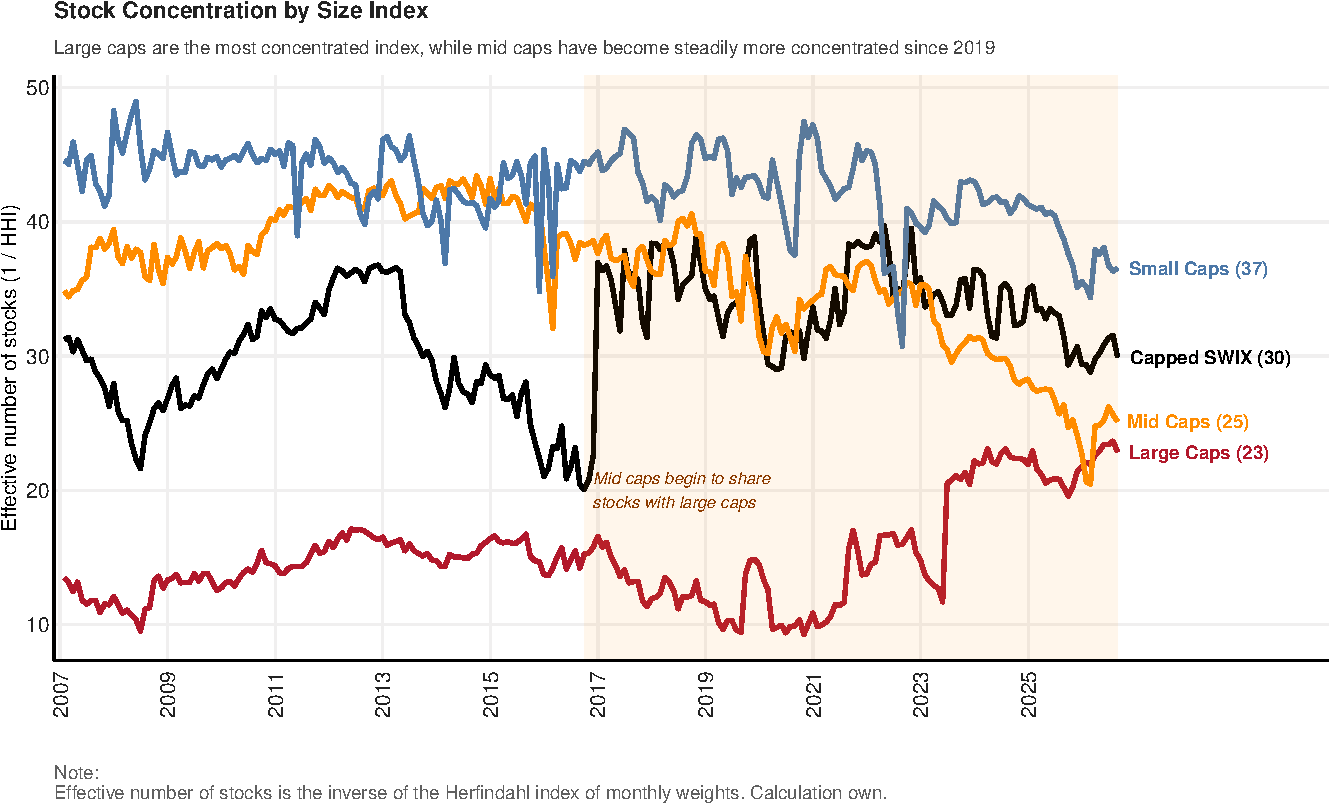
\includegraphics[width=1\linewidth]{Question2_files/figure-latex/q2_concentration-1} 

}

\caption{Stock Concentration by Size Index}\label{fig:q2_concentration}
\end{figure}

Concentration falls as company size falls. The large-cap index has
averaged an effective number of only 15 stocks, with 66 percent of its
weight in its ten largest holdings, against 43 stocks and 35 percent for
the small caps. The jump in the large-cap line in June 2023 comes from a
single stock, as Richemont's weight fell from 24 percent to 4 percent of
the index in one month, which lifted the effective number of stocks to
above 20 and left the large caps far less exposed to one company. The
mid caps moved the other way. Their effective number of stocks fell from
35 in 2007 to 25 in 2026, close to the large caps. From September 2016
the mid-cap index also began to hold stocks that sit in the large-cap
index, starting with 3 names, and by August 2026 the 14 shared names
made up 63 percent of mid-cap weight. The mid-cap index has therefore
become less distinct from the large caps in both its concentration and
its holdings, which matters for an investor who buys it as a separate
source of return.

\subsection{Active Share Against the Capped
SWIX}\label{active-share-against-the-capped-swix}

Active share measures how far an index's holdings differ from the
benchmark, as half the sum of absolute weight differences across all
stocks. A value of zero means identical holdings, while a value of one
means that the two hold no stock in common. It measures directly whether
a size index offers something the Capped SWIX does not.

\begin{figure}[H]

{\centering 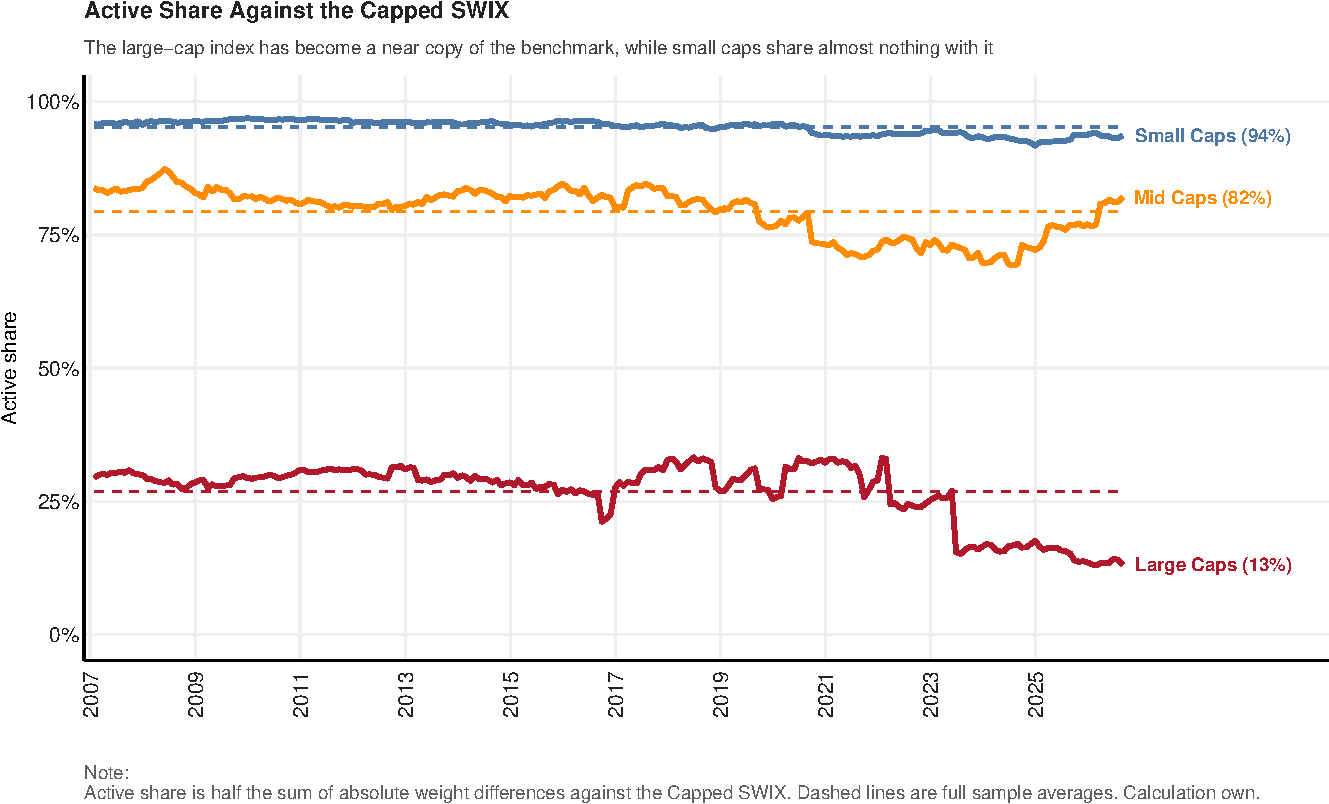
\includegraphics[width=1\linewidth]{Question2_files/figure-latex/q2_active_share-1} 

}

\caption{Active Share Against the Capped SWIX}\label{fig:q2_active_share}
\end{figure}

The three indexes sit at very different distances from the benchmark.
The large caps averaged an active share of 29 percent before June 2023
and only 15 percent after it, the same Richemont reweighting that
changed their concentration. At 13 percent in August 2026, the large-cap
index is close to a copy of the Capped SWIX, which is expected given
that the largest 40 stocks make up most of the benchmark's weight. The
mid caps averaged 79 percent, with a dip to around 70 percent between
2021 and 2024 that matches their growing overlap with the large caps.
The small caps averaged 95 percent, so almost all of their weight sits
in stocks that are tiny or absent in the benchmark. Of the three, only
the small caps offer a portfolio that is materially different from the
Capped SWIX, and their risk and return should be judged with that in
mind.

\section{\texorpdfstring{Realised Volatility of the Constituents
\label{Vol}}{Realised Volatility of the Constituents }}\label{realised-volatility-of-the-constituents}

\subsection{Constituent and Index
Volatility}\label{constituent-and-index-volatility}

The holdings are now combined with the daily stock returns to measure
how volatile each index's constituents are through time. At every month
end from April 2015, the realised volatility of each constituent is
measured over the trailing 63 trading days and averaged using the index
weights. The same weights are applied to the daily returns to form the
index return, whose realised volatility is measured over the same
window. The ratio of the two is the diversification ratio, which shows
how much of the stand-alone risk of the stocks disappears once they are
held together. Daily stock returns larger than 25 percent in absolute
value are winsorised, and a month is used only when at least 80 percent
of the index weight has return data.

\begin{figure}[H]

{\centering 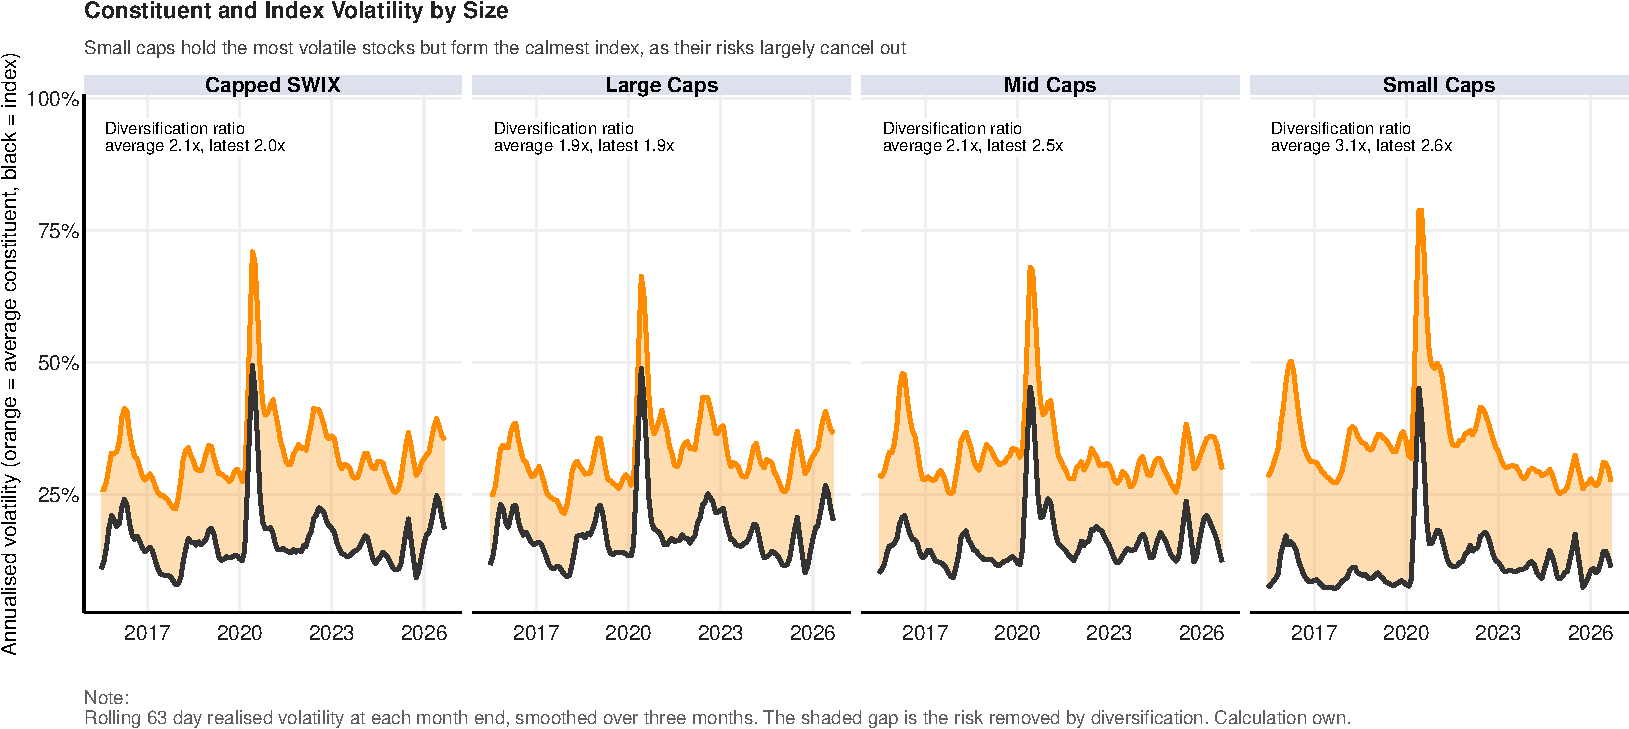
\includegraphics[width=1\linewidth]{Question2_files/figure-latex/q2_volatility-1} 

}

\caption{Constituent and Index Volatility by Size}\label{fig:q2_volatility}
\end{figure}

The figure shows the most distinctive trait of the small caps. Their
constituents are the most volatile of the three indexes, at an average
of 35 percent against 33 percent for the large caps, yet the small-cap
index is the calmest, at 12 percent against 18 percent. The
diversification ratio of the small caps averaged 3.1 against 1.9 for the
large caps. Small-cap stocks are driven mostly by their own news, such
as a single property portfolio or a regional retailer, so their shocks
are largely unrelated and cancel out inside the index. Large-cap stocks
share common drivers, namely commodity prices, the rand and global risk
appetite, so far less of their risk diversifies away.

That benefit is not stable. During the Covid crash between March and
June 2020, average small-cap stock volatility reached 77 percent and the
diversification ratio fell to 1.9, as every stock fell together. In 2026
the pattern reversed between sizes. The gold miners pushed average
large-cap stock volatility to 38 percent, above the 29 percent of
small-cap stocks, while the small-cap diversification ratio slipped to
2.4 from 3.1 in other months.

\subsection{Thin Trading and Measured
Volatility}\label{thin-trading-and-measured-volatility}

Part of the small caps' calm is also a measurement effect. Small stocks
trade thinly, so their prices often go unchanged for days and then catch
up, which smooths daily returns and understates volatility measured from
them.

The published small-cap index has a first order autocorrelation of 0.15
in its monthly returns, against -0.08 for the large caps. It is also the
only index whose volatility is higher when measured from monthly
returns, at 15.0 percent, than from daily returns, at 14.0 percent,
while the large caps show the reverse. Both are the signature of stale
prices, so the daily figures above flatter the small caps somewhat and
their true volatility sits closer to that of the other indexes.

The large caps show the reverse pattern. Their volatility from monthly
returns, at 15.1 percent, is below their volatility from daily returns,
at 18.7 percent, which is consistent with the slight negative
autocorrelation of -0.08 expected in a liquid index whose daily
overreactions partly reverse. The size of the gap between the two
measures therefore gives a rough guide to how much each index's daily
volatility should be adjusted.

\section{\texorpdfstring{Risk and Return Profiles
\label{Returns}}{Risk and Return Profiles }}\label{risk-and-return-profiles}

\subsection{Full Sample and Sub-Period
Profiles}\label{full-sample-and-sub-period-profiles}

The published indexes give a full record of returns from January 2015 to
September 2026. Each size index is measured against the Capped SWIX,
with the STeFI as the risk free rate, and the full sample is then split
into three sub-periods. These are the weak years before Covid, the Covid
crash and recovery between 2020 and 2022, and the recent period from
2023.

\begin{figure}[H]

{\centering 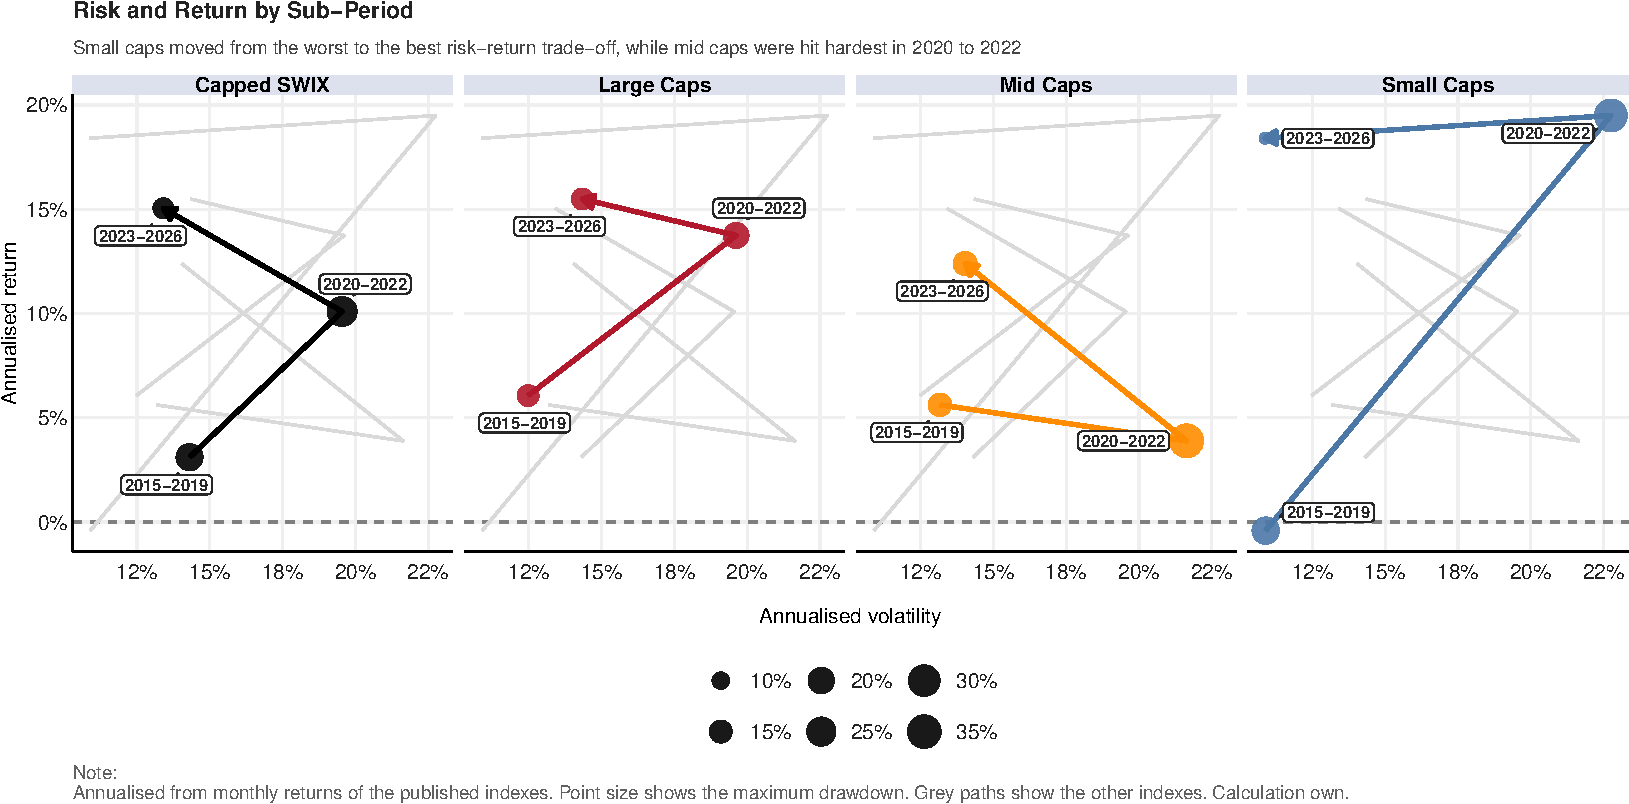
\includegraphics[width=1\linewidth]{Question2_files/figure-latex/q2_risk_return-1} 

}

\caption{Risk and Return by Sub-Period}\label{fig:q2_risk_return}
\end{figure}

Over the full sample, the large caps delivered the best trade-off, with
an annualised return of 10.9 percent, a Sharpe ratio of 0.77 and the
shallowest maximum drawdown, at 19.9 percent. The small caps earned
almost as much, at 10.3 percent, with a beta of only 0.68 and a down
capture of 0.48, so on average they lost less than half of what the
benchmark lost in its down months. Their bear market beta of 1.03 points
to a weakness, however. In ordinary down months small caps hold up, but
in a deep sell-off they fall one for one with the market, which is how
they suffered the largest drawdown of any index, at 45.6 percent. The
mid caps were the weakest, with a return of 7.3 percent, a Sharpe ratio
of 0.53 and the worst asymmetry of all, a bull beta of 0.55 against a
bear beta of 1.07.

The sub-periods show that these averages hide large shifts. The small
caps returned -0.4 percent a year between 2015 and 2019, the worst of
any index, then 19.5 percent in the volatile recovery, and 18.4 percent
since 2023 with volatility of only 10.9 percent and a maximum drawdown
of 8.2 percent, the best profile of any index in any period. The mid
caps were hit hardest between 2020 and 2022, earning 3.9 percent with a
drawdown of 35.6 percent. The returns of the large caps improved
steadily across all three periods.

\subsection{Downside Risk}\label{downside-risk}

The full sample statistics above give one measure of each kind of loss.
A downside risk table adds several more, and the dot plots below rank
the indexes on each.

\begin{figure}[H]

{\centering 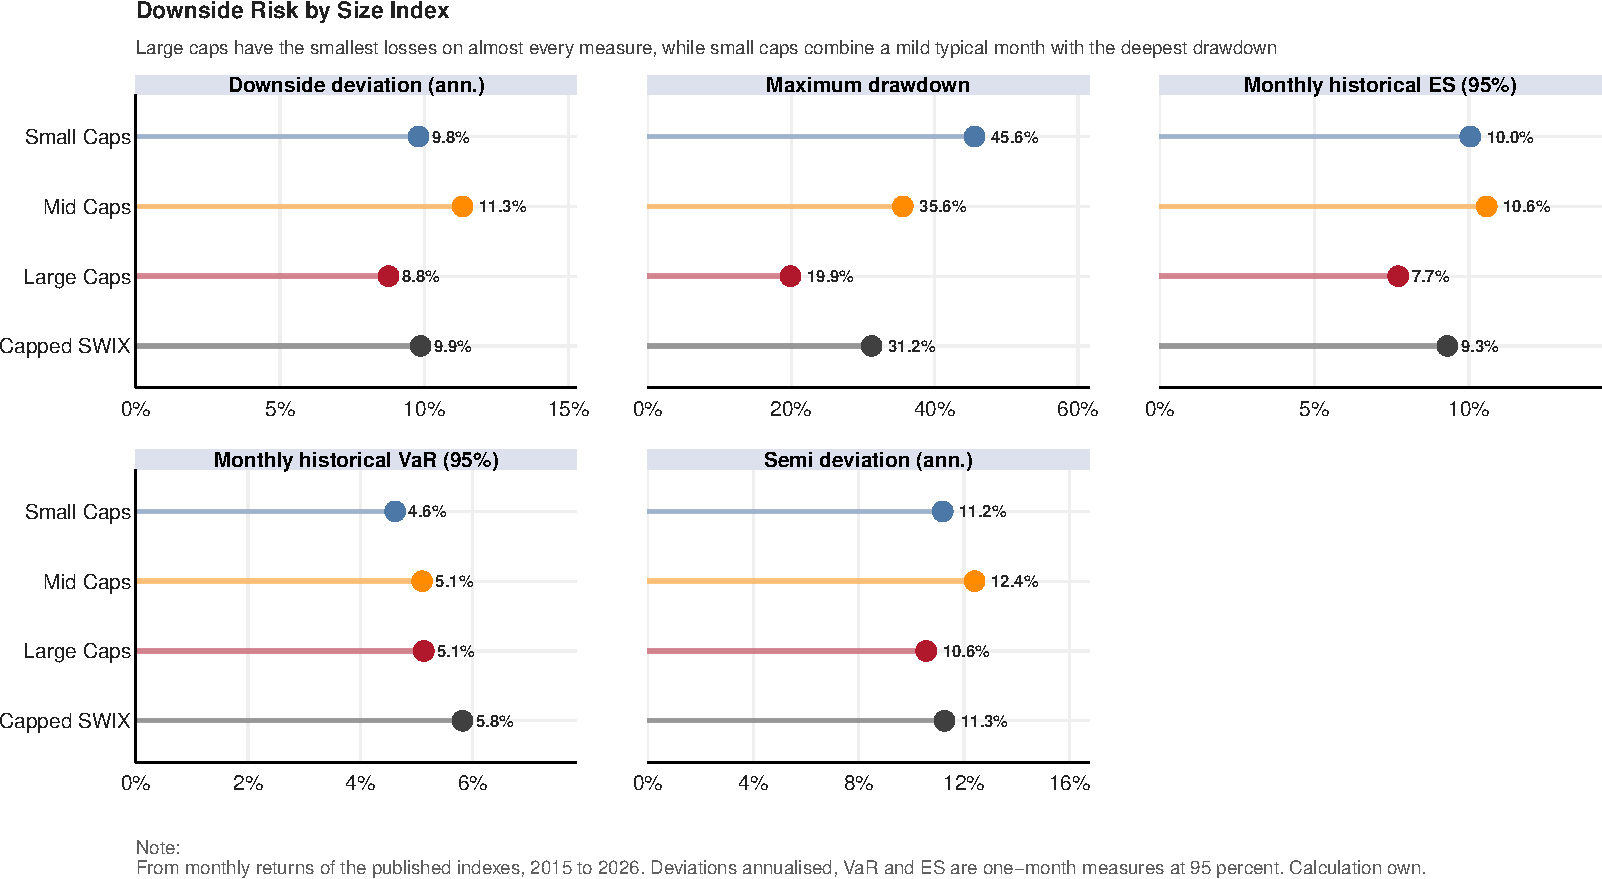
\includegraphics[width=1\linewidth]{Question2_files/figure-latex/q2_downside-1} 

}

\caption{Downside Risk by Size Index}\label{fig:q2_downside}
\end{figure}

The large caps have the mildest downside on four of the five measures,
with a downside deviation of 8.8 percent and a monthly expected
shortfall of 7.7 percent. The mid caps are the worst on downside
deviation, semi deviation and expected shortfall, at 10.6 percent for
the last. The small caps show the clearest contrast between measures.
Their monthly VaR is the lowest of all, at 4.6 percent, yet their
maximum drawdown is the deepest, at 45.6 percent. Losses that are small
in a typical bad month but run on for many months are consistent with
the positive autocorrelation and stale prices found above, and they show
why the small caps' low measured volatility should not be read as low
risk.

The ranking of the small caps depends on the measure chosen. Their semi
deviation of 11.2 percent is close to the large caps' 10.6 percent, yet
their drawdown is more than twice as deep, at 45.6 percent against 19.9
percent, because modest losses that persist across many months compound.
Which measure matters depends on the investor. A client who may need to
sell after a long fall faces the drawdown, while the monthly measures
describe the experience of an investor who stays the course.

\subsection{Rolling Returns}\label{rolling-returns}

Rolling returns show how the ranking of the indexes has changed from one
investment horizon to the next. The figure plots rolling three year
annualised returns and shades the months in which small caps were ahead
of large caps.

\begin{figure}[H]

{\centering 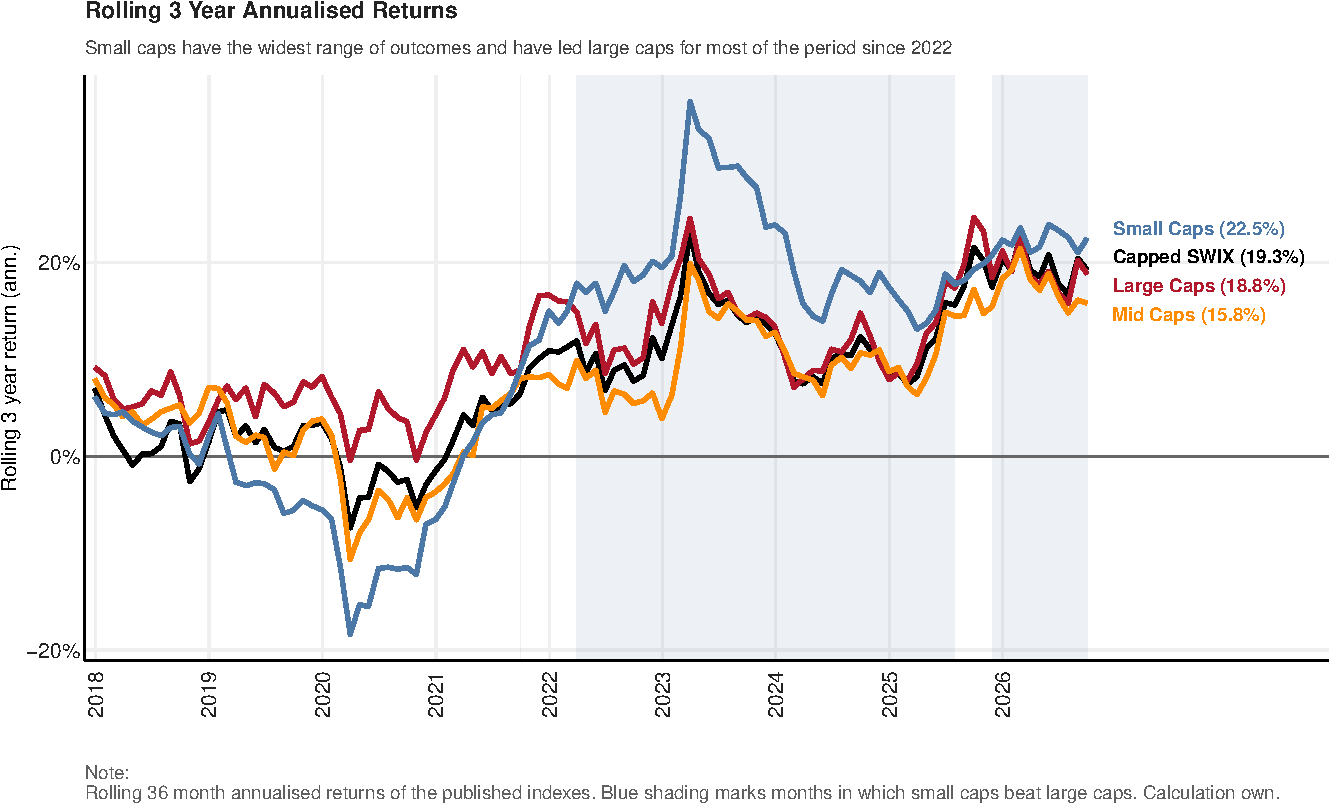
\includegraphics[width=1\linewidth]{Question2_files/figure-latex/q2_rolling-1} 

}

\caption{Rolling 3 Year Annualised Returns}\label{fig:q2_rolling}
\end{figure}

Small caps have the widest range of three year outcomes, from -18.4
percent in March 2020 to 36.6 percent in March 2023, while the worst
three year return of the large caps was -0.4 percent. An investor who
bought small caps in early 2017 and held them for three years would have
lost money, even though the index looked calm on a daily basis
throughout. The two segments led in turn, with small caps ahead in 50
percent of months, 98 percent of them from 2022 onwards. The rolling
returns of small and large caps have a correlation of 0.82, the lowest
of any pair, so over a three year horizon the small caps are the size
segment that most changes the outcome of a portfolio built around the
benchmark.

The widest gap between the two segments opened in March 2023, when the
small caps' three year return of 36.6 percent compared with 24.6 percent
for the large caps. Since then the two series have converged, and by
September 2026 the small caps' rolling return of 22.5 percent was only
modestly above the large caps' 18.8 percent.

\subsection{Returns Over Different
Horizons}\label{returns-over-different-horizons}

Annualised returns over several trailing horizons show whether a ranking
depends on the period chosen. The bars below end in September 2026, with
returns over one year or less shown as cumulative and longer horizons
annualised.

\begin{figure}[H]

{\centering 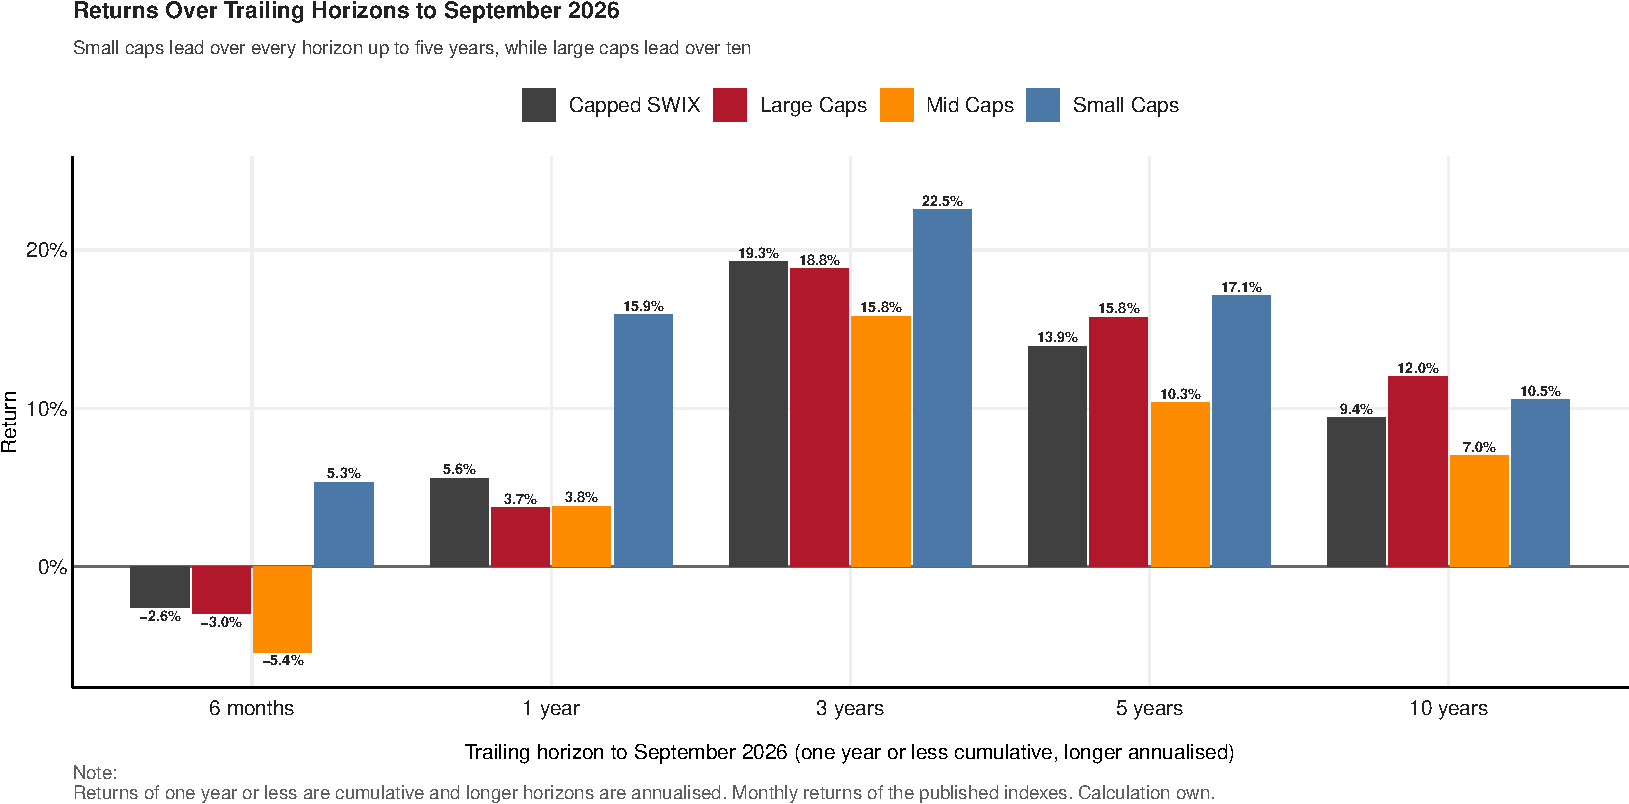
\includegraphics[width=1\linewidth]{Question2_files/figure-latex/q2_horizons-1} 

}

\caption{Returns Over Trailing Horizons to September 2026}\label{fig:q2_horizons}
\end{figure}

The ranking depends on the horizon. Over the past six months the small
caps gained 5.3 percent while every other index lost money, and over one
year they returned 15.9 percent against 3.7 percent for the large caps.
Their lead holds over three and five years, at 17.1 percent a year over
five years. Over ten years, however, the large caps lead, at 12.0
percent a year against 10.5 percent, because the ten year window still
contains the weak years of 2016 to 2020 seen in the rolling returns. The
mid caps are last over every horizon except one year, where the large
caps trail them by a fraction of a point.

The five year horizon, which begins after the weak years before 2020,
gives the small caps a lead of 1.4 percentage points a year over the
large caps. The ten year horizon, which starts in October 2016, still
includes most of the period from 2015 to 2019, in which the small caps
returned -0.4 percent a year, so the choice of horizon alone is enough
to reverse the ranking of the two segments.

\section{\texorpdfstring{Behaviour Across Market Regimes
\label{Strat}}{Behaviour Across Market Regimes }}\label{behaviour-across-market-regimes}

\subsection{Calm and Stressed Months}\label{calm-and-stressed-months}

The final step asks how each index behaves in different market
conditions. Months are sorted into quintiles of three state variables,
and the annualised return and volatility of each index are compared
between the bottom and top quintile. The state variables are the monthly
return of the Capped SWIX, rand volatility measured by the monthly
average of the SAVIUSD index, and global risk aversion measured by the
monthly average of the VIX.

\begin{figure}[H]

{\centering 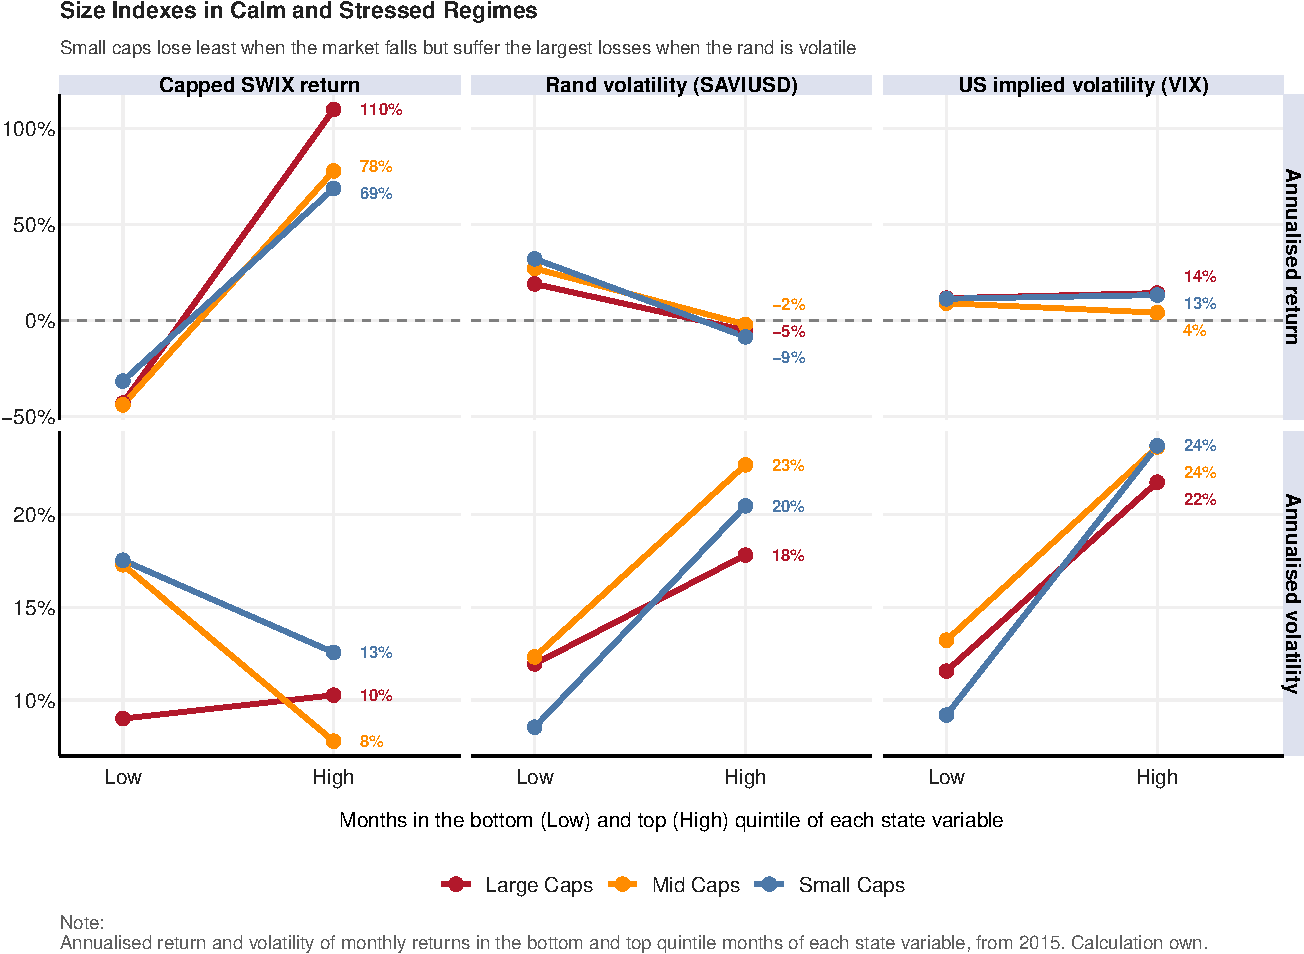
\includegraphics[width=1\linewidth]{Question2_files/figure-latex/q2_stratify-1} 

}

\caption{Size Indexes in Calm and Stressed Regimes}\label{fig:q2_stratify}
\end{figure}

Each quintile contains 29 months. The stratification adds detail to the
capture statistics. In the worst fifth of months for the benchmark, the
small caps lost at an annualised rate of -32 percent, against -43
percent for the large caps, but with nearly twice the volatility, at 18
percent against 9 percent. Their protection in falling markets is
therefore real on average but unreliable from month to month. In the
best fifth of months the large caps gained most, at 110 percent, which
is the mirror image of the small caps' low beta.

Rand volatility is the state that separates the indexes most clearly.
When the rand is calm, small caps are the best performer, at 32 percent,
with the lowest volatility of the three in that regime. When the rand is
volatile they become the worst, at -9 percent, with volatility more than
doubling. That pattern fits their domestic sector mix, since a volatile
rand signals local stress and raises imported inflation and interest
rate risk, while the large caps' offshore earnings and resource exports
act as a partial hedge. The VIX, by contrast, barely changes returns. It
raises the volatility of every index, and most of all for small caps,
whose volatility rises from 9 percent to 24 percent, while the mid caps
alone see their return fall sharply, to 4 percent.

\FloatBarrier

\section{\texorpdfstring{Conclusion
\label{Conclusion}}{Conclusion }}\label{conclusion}

The three size indexes offer very different exposures within the same
market. The large-cap index is a concentrated, resource-heavy portfolio
that has become close to a copy of the Capped SWIX, with an active share
of 13 percent. Its risk comes from common global drivers that diversify
poorly, but it has delivered the best full-sample trade-off and the
shallowest drawdowns. The small-cap index is the only one that is
materially different from the benchmark. It is a domestic,
property-heavy portfolio of volatile but largely unrelated stocks, which
makes the index calm in ordinary times and leaves it exposed in crises,
in deep sell-offs and in periods of rand stress, when its
diversification breaks down. Its low measured volatility is also partly
an artefact of thin trading. The mid-cap index has drifted towards the
large caps in its holdings and concentration, and has offered the
weakest return and the least favourable asymmetry between up and down
markets.

For an investor, the indexes are therefore not interchangeable ways of
owning local equity. The large caps are effectively the benchmark. The
small caps add diversification and have rewarded patience since 2022,
but they should be sized for their crisis behaviour and their dependence
on domestic conditions, and the calm suggested by their daily volatility
should not be taken at face value.

\bibliography{Tex/ref}





\end{document}
